\documentclass[12pt]{amsart}

% ===== Packages =====
\usepackage{amsmath,amssymb,amsthm,mathtools}
\usepackage[margin=1in]{geometry}
\usepackage{microtype}
\usepackage{enumitem}
\usepackage{tikz}
\usetikzlibrary{arrows.meta,positioning}
\usepackage[colorlinks=true,linkcolor=blue,citecolor=blue,urlcolor=blue]{hyperref}

% ===== Theorem Environments =====
\numberwithin{equation}{section}
\newtheorem{theorem}{Theorem}[section]
\newtheorem{proposition}[theorem]{Proposition}
\newtheorem{lemma}[theorem]{Lemma}
\newtheorem{corollary}[theorem]{Corollary}
\newtheorem{assumption}[theorem]{Assumption}
\theoremstyle{definition}
\newtheorem{definition}[theorem]{Definition}
\theoremstyle{remark}
\newtheorem{remark}[theorem]{Remark}
\newtheorem{principle}[theorem]{Design Principle}

% ===== Macros =====
\newcommand{\PP}{\mathcal P}
\newcommand{\RRc}{\mathcal R}
\newcommand{\II}{\mathcal I}
\newcommand{\KK}{\mathcal K}
\newcommand{\GG}{\mathcal G}
\newcommand{\CC}{\mathcal C}
\newcommand{\YY}{Y}
\newcommand{\TT}{\mathcal T}

\title{Proof-Carrying Cognition:\\
A Domain-Agnostic Admissibility Kernel}
\author{Jean Marie Tassy Simeoni}
\date{}

\begin{document}
\maketitle

\begin{abstract}
We introduce a domain-agnostic admissibility architecture for converting speculative, generative,
or heuristic internal structure into externally admissible artifacts.  The central claim is that
internal coherence, richness, or explanatory appeal do not suffice for admissibility.  Rather, an
object becomes admissible only after crossing a deterministic transmutation boundary governed by
receipts, invariants, and fail-closed gates.

Formally, we define an admissibility kernel as a 5-tuple
\[
  \mathfrak A=(\PP,\RRc,\II,\KK,\GG),
\]
where $\PP$ is a proposal space, $\RRc$ a receipt space, $\II$ a family of invariants, $\KK$ a
deterministic reducer, and $\GG$ a gate system.  We factor admissibility through an evaluation
space $\YY$:
\[
  \KK:\PP\times\RRc\to \YY, \qquad \GG:\YY\to \CC\cup\{\bot\},
\]
so that the induced transmutation operator is
\[
  \TT_{\mathfrak A}=\GG\circ\KK:\PP\times\RRc\to\CC\cup\{\bot\}.
\]
The framework does not claim metaphysical truth.  It formalizes a weaker and more operational
notion: permission for a generated structure to count under a declared contract.
\end{abstract}

% ------------------------------------------------------------------
\section{Introduction}
% ------------------------------------------------------------------

The production of internal structure is cheap.  Mathematical, computational, and cognitive systems
can generate candidate constructions, conjectural mechanisms, plans, narratives, and symbolic
correspondences at a rate far exceeding the rate at which any of these may reasonably be trusted.
The bottleneck is therefore not generation, but admissibility.

This asymmetry recurs across apparently distant domains.  In exploratory mathematics, elegant
operators, suggestive correspondences, or compelling numerical patterns do not thereby become
theorem-level claims.  In software and multi-agent systems, polished reports and coherent summaries
do not thereby become grounded outputs.  In governance-like computational systems, a proposal may
be articulate, internally consistent, and rhetorically strong while remaining non-sovereign unless
it survives receipt-bound reduction.

The claim of this paper is that these are not merely analogies.  They instantiate a common
architectural pattern: admissibility is itself an operator-governed boundary.  The primary object
is therefore not merely the generated theory, plan, or artifact, but the kernel that decides
whether such an object is permitted to count.

% ------------------------------------------------------------------
\section{The Admissibility Kernel}
% ------------------------------------------------------------------

\begin{definition}[Proposal space]
A \emph{proposal space} $\PP$ is a class of internally generated objects.  Its elements possess
no default authority.
\end{definition}

\begin{definition}[Receipt space]
A \emph{receipt space} $\RRc$ is a class of externally inspectable witnesses sufficient to support
deterministic recomputation.  Receipts are replayable witnesses, not explanations.
\end{definition}

\begin{definition}[Invariant family]
An \emph{invariant family} $\II$ is a collection of predicates or structured constraints declared
by contract.
\end{definition}

\begin{definition}[Evaluation space]
An \emph{evaluation space} $\YY$ is the codomain of admissibility-relevant reducer state.
Typical examples include vectors of gate checks, structured diagnostics, typed obligation states,
or bounded score tuples.  $\YY$ is distinct from both the proposal and the certified artifact
space; it is the intermediate record of what the reducer observed.
\end{definition}

\begin{definition}[Deterministic reducer]
A \emph{deterministic reducer} is a map
\[
  \KK:\PP\times\RRc\to\YY
\]
whose defining property is that identical declared inputs produce identical outputs.
\end{definition}

\begin{definition}[Gate system]
A \emph{gate system} is a map
\[
  \GG:\YY\to\CC\cup\{\bot\},
\]
or equivalently a finite family of predicates on $\YY$ whose aggregate action determines
admissibility.  $\bot$ denotes rejection.
\end{definition}

\begin{definition}[Certified artifact space]
A \emph{certified artifact space} $\CC$ is the codomain of externally admissible objects.
\end{definition}

\begin{definition}[Transmutation operator]
Given $\mathfrak A=(\PP,\RRc,\II,\KK,\GG)$, the induced \emph{transmutation operator} is
\[
  \TT_{\mathfrak A}=\GG\circ\KK:\PP\times\RRc\to\CC\cup\{\bot\}.
\]
\end{definition}

\subsection*{Factorization diagram}

\[
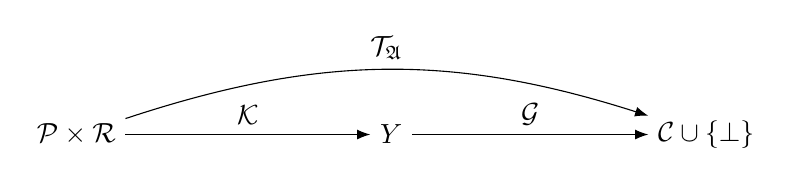
\begin{tikzpicture}[baseline=(current bounding box.center),>=Latex]
  \node (PR) at (0,0)  {$\PP\times\RRc$};
  \node (Y)  at (4,0)  {$\YY$};
  \node (C)  at (8,0)  {$\CC\cup\{\bot\}$};

  \draw[->] (PR) -- node[above] {$\KK$} (Y);
  \draw[->] (Y)  -- node[above] {$\GG$} (C);
  \draw[->,bend left=18] (PR) to node[above] {$\TT_{\mathfrak A}$} (C);
\end{tikzpicture}
\]

% ------------------------------------------------------------------
\section{Axioms of Admissibility}
% ------------------------------------------------------------------

\begin{assumption}[No default authority]
No element of proposal space is admissible by default.
\end{assumption}

\begin{assumption}[Receipt grounding]
Every admissible artifact must be grounded in a receipt structure sufficient for kernel-side
recomputation.
\end{assumption}

\begin{assumption}[Deterministic recomputation]
The reducer $\KK$ is deterministic on declared inputs.
\end{assumption}

\begin{assumption}[Fail-closed boundary]
Failure of receipts, invariants, or gates yields $\bot$.
\end{assumption}

\begin{assumption}[Scoped admissibility]
Admissibility is contract-relative and does not imply metaphysical truth.
\end{assumption}

% ------------------------------------------------------------------
\section{General Structural Properties}
% ------------------------------------------------------------------

\begin{proposition}[Narrative non-sovereignty]
Narrative content may enlarge proposal space $\PP$, but it cannot enlarge certified artifact
space $\CC$ without corresponding receipt and gate satisfaction.
\end{proposition}

\begin{proof}
By no default authority, narrative has no direct admissibility force.  By receipt grounding,
admissibility requires recomputable witness structure.  By fail-closed boundary, unsatisfied
receipt or gate conditions yield $\bot$.
\end{proof}

\begin{proposition}[Controlled extensivity under added receipts]
Under fixed reducer and gate semantics, enlarging receipt space may enlarge the admissible set
or leave it unchanged, but it cannot bypass recomputation.
\end{proposition}

\begin{proof}
Any effect of additional receipts is mediated through $\KK$ and then $\GG$.  No alternate
admissibility path exists by definition of $\TT_{\mathfrak A}$.
\end{proof}

\begin{principle}[Small-gate-surface]
Gate vocabulary should remain small even when proposal payloads and receipt structures grow
richer.  A large gate surface increases the attack area for admissibility laundering.
\end{principle}

\begin{remark}
The small-gate-surface principle is an architectural design choice, not a consequence of the
axioms.  Systems that violate it remain formally consistent with the kernel definition; they
are merely more difficult to audit and replay.
\end{remark}

% ------------------------------------------------------------------
\section{Admissibility as the Main Object}
% ------------------------------------------------------------------

\begin{theorem}[Admissibility principle]
Let a domain be equipped with a declared proposal space $\PP$, receipt space $\RRc$, invariant
family $\II$, deterministic reducer $\KK$, and gate system $\GG$.  Then the externally admissible
artifacts in that domain are exactly those surviving recomputation under the induced transmutation
operator $\TT_{\mathfrak A}$.
\end{theorem}

\begin{proof}
By no default authority, no proposal is admissible by default.  By receipt grounding and
deterministic recomputation, admissibility is decided only through reducer-side evaluation on
declared inputs.  By fail-closed boundary, failed evaluation yields $\bot$.  Hence admissibility
is exactly the image of $\TT_{\mathfrak A}$ outside $\bot$.
\end{proof}

\begin{corollary}[Content is abundant, admissibility is scarce]
Increasing generative richness enlarges proposal space, while admissible artifacts remain
constrained by receipts, invariants, and gates.
\end{corollary}

% ------------------------------------------------------------------
\section{Instantiations}
% ------------------------------------------------------------------

We give two compact typed instantiations.  Each demonstrates that the formal vocabulary of
Section~2 applies directly to deployed systems, and that the boundaries between $\PP$, $\YY$,
and $\CC$ are implementable distinctions, not merely notational ones.

\subsection{Receipt-Governed Governance (HELEN OS)}

In the HELEN OS governance architecture, the five components of the admissibility kernel
instantiate as follows.

\begin{itemize}[leftmargin=2em]
  \item $\PP$: \texttt{HELEN\_CONCLUSION\_V1} artifacts — non-authoritative proposal objects
    emitted by the HELEN cognitive layer.  Each carries a declared \texttt{shipability} value
    fixed at \texttt{NONSHIPABLE} by construction.

  \item $\RRc$: \texttt{AUTHZ\_RECEIPT\_V1} objects, gate receipts, and evaluation receipts.
    Each receipt binds to a specific \texttt{(verdict\_id, verdict\_hash\_hex)} pair computed
    by the kernel; receipt structure is sufficient for deterministic recomputation of the
    reduction.

  \item $\II$: The \textsc{Canyon Noninterference Law} — same evidence set $E_{\mathrm{adm}}$
    produces the same \texttt{verdict\_hash\_hex}.  Formally:
    \[
      E_{\mathrm{adm}} = E_{\mathrm{adm}}' \implies \KK(p, r) = \KK(p', r')
    \]
    for any proposals $p, p'$ agreeing on $E_{\mathrm{adm}}$.  Narrative variation in
    $p$ cannot alter the kernel output.

  \item $\YY$: A structured diagnostic tuple
    $(\texttt{gate\_checks}, \texttt{sigma\_value}, \texttt{metrics\_vector})$.
    Gate checks record pass/fail per gate; $\sigma$ is the normalized scalar derived from
    measurable predicates; metrics are bounded real values.  No wall-clock timestamp appears
    in $\YY$.

  \item $\GG$: Three sequential predicates — \textsc{MayorCheck} (authority scan),
    \textsc{AuthorityScan} (forbidden-token check), \textsc{SchemaValidation} —
    all of which must pass.  $\GG(\YY) \in \CC$ iff all three pass; otherwise $\bot$.

  \item $\CC$: SHIP-eligible artifacts, each carrying a sealed
    $\texttt{verdict\_hash\_hex} = \mathrm{SHA256}(\mathrm{canonical\_json}(
    \texttt{quest\_id}, \texttt{quest\_type}, \texttt{gates}, \texttt{next\_quest\_seed}))$.
\end{itemize}

The governance-side instance makes explicit the intended operational reading of the axioms:
\emph{no receipt $=$ no ship}.  An articulate HELEN proposal that satisfies no receipt
requirements is a proposal in $\PP$ only; it never reaches $\CC$.

\subsection{HELEN EPOCH3 Quest Reduction}

The EPOCH3 simulation loop provides a second, more computational instantiation focused on
deterministic quest evaluation without entropy injection.

\begin{itemize}[leftmargin=2em]
  \item $\PP$: Quest proposals of type
    $\{\texttt{Q1\_PARADOX},\, \texttt{Q2\_REALITY},\, \texttt{Q3\_TEMPORAL}\}$,
    each parameterized by a seed and a tick budget.

  \item $\RRc$: Ledger receipts with fields
    $(\texttt{payload\_hash},\, \texttt{cum\_hash})$ forming a hash chain under the rule
    $\texttt{cum\_hash}_n = \mathrm{SHA256}(\texttt{cum\_hash}_{n-1} \mathbin\| \texttt{payload\_hash}_n)$.
    No wall-clock value and no entropy source appears in $\RRc$.

  \item $\II$: Replay determinism — the kernel run with the same seed, tick count, and
    ledger tip produces byte-identical output.

  \item $\YY$: The \texttt{ReducedConclusion} object produced by
    $\texttt{ConclusionReducer.reduce(conclusion, sim\_result, kernel)}$, containing
    gate pass/fail indicators and a deterministic
    \[
      \texttt{next\_quest\_seed} =
        \mathrm{SHA256}(\texttt{quest\_id}
          \mathbin\| \mathrm{sorted}(\texttt{receipt\_pointers})
          \mathbin\| \mathrm{SHA256}(\mathrm{canonical\_json}(\texttt{gates}+\texttt{metrics}))).
    \]

  \item $\GG$: The sigma gate — a scalar threshold predicate on the normalized sigma value
    computed from measurable quest metrics.  Sigma $\geq$ threshold maps to $\CC$; otherwise
    $\bot$.

  \item $\CC$: Sealed \texttt{QuestResult} objects with frozen
    $\texttt{verdict\_hash\_hex}$, suitable for admission into the sovereign ledger.
\end{itemize}

In both instantiations, the evaluation space $\YY$ is the precise location at which the
system's decision-relevant state is made inspectable.  The gate system $\GG$ then acts on
$\YY$ alone; no path to $\CC$ bypasses this inspection point.

% ------------------------------------------------------------------
\section{Limits and Non-Claims}
% ------------------------------------------------------------------

Admissibility is not the same as truth.  Passing through one admissibility kernel does not
imply admissibility under another.  The framework is only as strong as the instantiated
reducer, receipt discipline, and gate design.

The factorization $\TT_{\mathfrak A} = \GG \circ \KK$ is a structural decomposition, not a
decision procedure.  The difficulty of realizing a well-behaved kernel in any given domain is
not reduced by the formalism; only its desiderata are made explicit.

Scoped admissibility (Assumption~3.5) implies that a certified artifact carries authority only
within the declared contract.  Cross-domain or cross-kernel authority claims are not licensed
by the framework.

\end{document}
